\section{Chapter 3}\label{main_section_2}

% Example of an image with a footnote
\begin{figure}[htb]
    \centering
    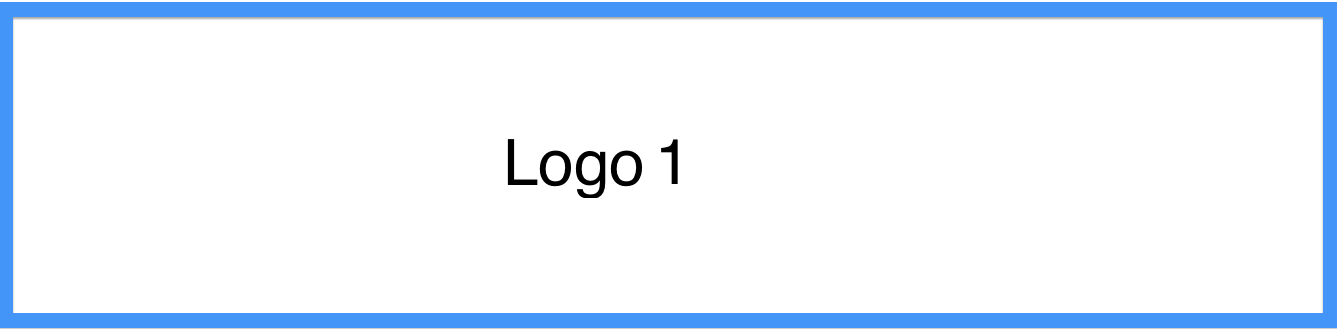
\includegraphics[width=0.4\textwidth,angle=45]{abb/logo1}
    \caption[Example of a figure description]{Example of a figure description\footnotemark}
    \label{fig:example1}
\end{figure}
\footnotetext{Image source: Example of an image source}

% Example of image integration
\begin{figure}[htb]
    \centering
    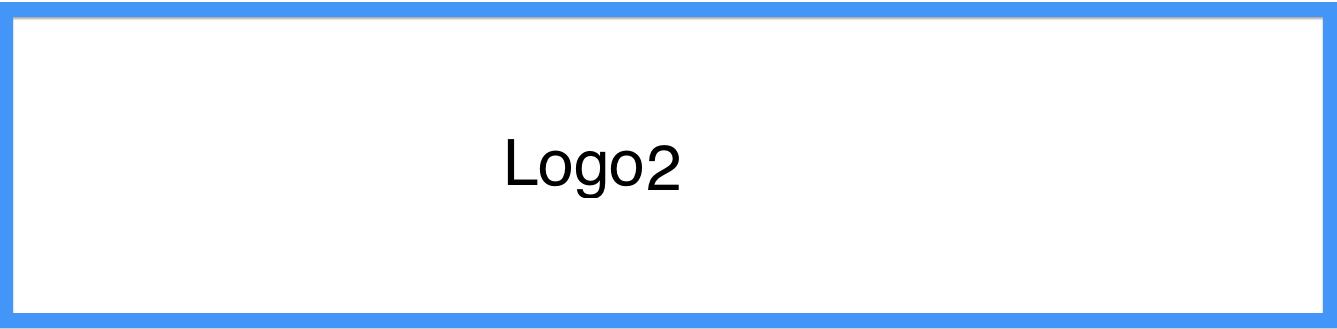
\includegraphics[width=0.3\textwidth,angle=0]{abb/logo2}
    \caption[Description]{Description \cite[p. 96]{mf2005}}
    \label{fig:description}
\end{figure}

% Example: Reference to figure
Figure~\ref{fig:description} [p.\pageref{fig:description}]

% Example: Table 
\begin{table}[!h]
    \begin{center}
        \begin{tabular}{ | l | c | }
            \hline
            Heading 1 & Heading 2 \\ \hline \hline
            Info 1 & Info 2 \\ \hline
            Info 3 & Info 4 \\ \hline
            \hline
            \multicolumn{2}{|c|}{Info in one cell} \\
            \hline
        \end{tabular}
        \caption[Description of the table]{Description of the table \cite[p. 13]{mm2009}}
    \end{center}
\end{table}


% Example for source code listings
\lstset{language=xml}
\begin{lstlisting}[frame=htrbl, caption={The file {\normalfont \ttfamily  data-config.xml} serves as an example for XML source code}, label={lst:dataconfigxml}]
    <dataConfig>
    <dataSource type="JdbcDataSource" 
    driver="com.mysql.jdbc.Driver"
    url="jdbc:mysql://localhost/bms_db"
    user="root" 
    password=""/>
    <document>
    <entity name="id"
    query="select id, htmlBody, sentDate, sentFrom, subject, textBody
    from mail">
    <field column="id" name="id"/>
    <field column="htmlBody" name="text"/>
    <field column="sentDate" name="sentDate"/>
    <field column="sentFrom" name="sentFrom"/>
    <field column="subject" name="subject"/>
    <field column="textBody" name="text"/>
    </entity>
    </document>
    </dataConfig>
\end{lstlisting}

\lstset{language=java}
\begin{lstlisting}[frame=htrbl, caption={This listing shows Java source code}, label={lst:result2}]
    /* generate TagCloud */
    Cloud cloud = new Cloud();
    cloud.setMaxWeight(_maxSizeOfText);
    cloud.setMinWeight(_minSizeOfText);
    cloud.setTagCase(Case.LOWER);
    
    /* evaluate context and find additional stopwords */
    String query = getContextQuery(_context);
    List<String> contextStoplist = new ArrayList<String>();
    contextStoplist = getStopwordsFromDB(query);
    
    /* append context stoplist */
    while(contextStoplist != null && !contextStoplist.isEmpty())
    _stoplist.add(contextStoplist.remove(0));
    
    /* add cloud filters */
    if (_stoplist != null) {
        DictionaryFilter df = new DictionaryFilter(_stoplist);
        cloud.addInputFilter(df);
    }
    /* remove empty tags */
    NonNullFilter<Tag> nnf = new NonNullFilter<Tag>();
    cloud.addInputFilter(nnf);
    
    /* set minimum tag length */
    MinLengthFilter mlf = new MinLengthFilter(_minTagLength);
    cloud.addInputFilter(mlf);
    
    /* add taglist to tagcloud */
    cloud.addText(_taglist);
    
    /* set number of shown tags */	    
    cloud.setMaxTagsToDisplay(_tagsToDisplay);
\end{lstlisting}


% Example for formulas
The assignment of all possible values that a random variable can take is called the \emph{distribution function} of $X$.

\begin{quotation}
    The function F: $\mathbb{R} \rightarrow$ [0,1] with $F(t) = P (X \le t)$ is called the distribution function of $X$ \cite[pp. 42--49]{mm2009}.
\end{quotation}

\begin{quotation}
    For a continuous random variable $X: \Omega \rightarrow \mathbb{R}$, an integrable, non-negative real function $w: \mathbb{R} \rightarrow \mathbb{R}$ with $F(x) = P(X \le x) = \int_{-\infty}^{x} w(t)dt$ is called the \emph{density} or \emph{probability density} of the random variable $X$.\footnote{Mustermann, see~\cite{mf2005}~[p.56]}
\end{quotation}
